\chapter{Orquestación de contenedores: Kubernetes}
\label{chap:kubernetes}

Los contenedores que hemos visto en el capítulo anterior es una tecnología excelente para nuestro propósito, pero se mueven en un sistema de abstracción demasiado bajo. Quiero aislar mi solución del proveedor hardware o cloud de turno y no quiero tener que administrar máquinas. Kubernetes me ayuda a formar ese plano de control de contenedores.

Kubernetes es un software que controla un cluster de máquinas estableciendo una capa de abstracción uniforme sobre ellas para que no tengamos que preocuparnos individualmente sobre ninguna, solo sobre el colectivo entero. Es lo que se denomina Mascotas versus Ganado\cite{noahslater2014} haciendo una referencia al modo de tratar a cada máquina. Esto es especialmente relevante en la nube donde podemos encender o apagar máquinas muy rápidamente según la carga o la necesidad de computación. Los contenedores facilitan la configuración de cada máquina (apenas deben tener Docker instalado) pero necesitamos una herramienta para controlarlas independientemente del tipo que sean y de los recursos que posean.

\section{Orígenes: Borg}
\label{sec:borg}

Kubernetes surge de un grupo de ingenieros de Google que deseaban disponer de una herramienta de código abierto que pudieran usar los clientes de Google Cloud y otros desarrolladores\cite{cademetz2015}. El objetivo era reusar todo los conocimientos que los ingenieros de Google poseían sobre la administración de contenedores de haber construido y mantenido su propia versión interna: Borg\cite{43438}. Reciclando algunos de los conceptos claves\cite{k8sborg} que posteriormente han dado forma al resto del sistema el proyecto tomó forma recientemente y se ha establecido como uno de los gestores de cluster más avanzados y completos del mercado, además de gratuito.

Al ser un proyecto de código abierto ha recibido contribuciones por parte de otras empresas líderes en el sector como RedHat, Fujitsu, IBM o CoreOS\cite{k8sanalytics} que han aportado fuerza de ingeniería para desarrollar nuevos componentes y características. Algunas ofrecen servicios específicos encima de la funcionalidad de Kubernetes como Red Hat con OpenShift\cite{openshift} y CoreOS con Tectonic\cite{tectonic}.

Una de las mayores diferencias con otras herramientas y que heredó de Borg es el bucle controlador de reconciliación\cite{borgomegak8s}. Este bucle se ejecuta constantemente y compara el estado deseado del sistema de acorde a los ficheros de configuración que tiene almacenados con el estado actual del sistema basado en las lecturas de demonios y otras fuentes. Si ese estado difiere con el deseado se toman medidas para corregirlo y llevarlo al rumbo correcto de nuevo. Por ejemplo, podemos decirle que deseamos que haya 3 instancias abiertas. Si en estos momentos hay 4 se tomarán medidas correctoras apagando una de ellas para llegar al estado deseado. Si de repente una de las instancias fallara y se apagara, se tomarían medidas para abrir otra nueva y volver al punto de control de nuevo. En cierto sentido es parecido al bucle de control cerrado del que hablaríamos si fuera un proyecto de robótica.

\section{Instalación}
\label{sec:k8s-install}

Podría pensarse que Google liberó conocimientos como herramienta para obtener más clientes en su nube; nada más lejos de la realidad. Kubernetes incorpora scripts\cite{clusterscripts} vetados y mantenidos por ellos mismos para auto instalarse con un comando en las plataformas en la nube (Google Cloud, Amazon AWs, Microsoft Azure, ...) y por demanda (Juju, Mesos, vSphere, ...) más conocidas. Una vez instalado el sistema abstrae de las diferencias entre máquinas y proporciona unas funcionalidades similares o parecidas esté donde esté.

\section{Estructura}
\label{sec:k8s-estructura}

Kubernetes está formado por 5 demonios con funciones diferentes (ver figura \ref{fig:k8s-arch}) e independientes\cite{k8sdesignarch}. Una de las máquinas del cluster (o varias si pensamos hacer una instalación de alta disponibilidad) contendrá algunos demonios especiales y no ejecutará ningún contenedor, solamente se dedicará a controlar al resto. Esta máquina es el \emph{master}, y el resto son \emph{nodos}.

\begin{figure}[H]
    \centering
    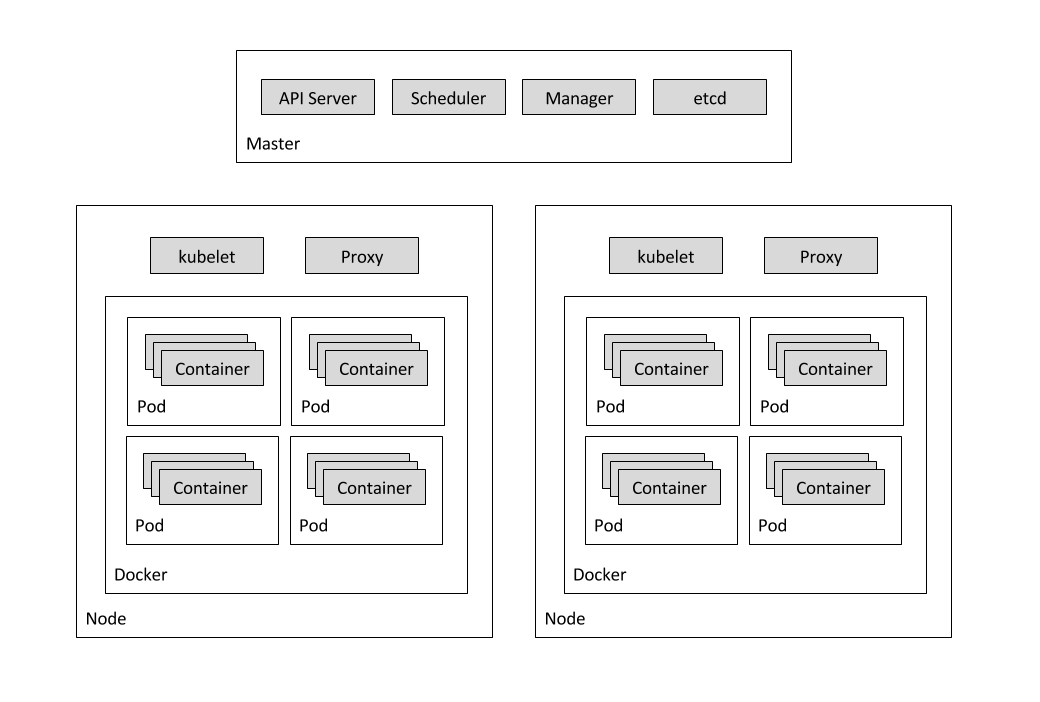
\includegraphics[width=\textwidth]{../images/kubernetes/arch.png}
    \caption{Diagrama de la arquitectura de demonios de Kubernetes \protect\cite{k8sarch}}
    \label{fig:k8s-arch}
\end{figure}

\subsection{Demonios del master}
\label{subsec:k8s-demonios-master}

\subsubsection{kube-apiserver}
\label{subsubsec:k8s-apiserver}

El corazón de un sistema de Kubernetes es el demonio que almacena y proporciona datos al resto de demonios. Las tareas del servidor de la API son:
\begin{itemize}
    \item Autenticar las peticiones de acorde a los usuarios y cuentas de servicio que existan.
    \item autorizar las operaciones según el nivel de acceso.
    \item Validar y guardar los datos de componentes para crearlos o actualizarlos.
    \item Almacenar permanentemente los datos de esos componentes de forma durable.
    \item Proveer de la información necesaria al resto de demonios para su buen funcionamiento.
\end{itemize}

Provee una API REST documentada\cite{k8sapi} a la que cualquiera con los permisos puede acceder. En mi trabajo accedo a esa API para crear nuevos objetos y que Kubernetes se encargue de configurar los servicios por mí en las máquinas disponibles.

\subsubsection{etcd}
\label{subsubsec:k8s-etcd}

Para el almacenamiento persistente y durable de los datos se usa una instancia de una base de datos llamada etcd. Almacena claves y valores \cite{etcd} solamente. Se puede replicar fácilmente entre varias máquinas usando un protocolo de sincronización conocido como Raft\cite{raft2013}. Se usa de forma interna por el servidor de la API y no se permite el acceso desde ningún otro componente del sistema para preservar la seguridad y la integridad.

\subsubsection{kube-controller-manager}
\label{subsubsec:k8s-controller-manager}

Observa cambios en la configuración para aplicarlos sobre las máquinas con el objetivo de alcanzar el estado deseado. Implementa el bucle controlador de reconciliación que mencioné antes. Algunos ejemplos de su actuación:
\begin{itemize}
  \item Controla el número de replicas para subir o bajar el número de contenedores activos de acuerdo a la configuración. La configuración a su vez puede cambiarse manualmente o automáticamente basándose en métricas (autoescalado horizontal).
  \item Si estamos en una plataforma en la nube como Google Cloud o Amazon AWS hay que mover los discos a las máquinas que estén ejecutando los contenedores que los necesitan.
  \item Cambia configuraciones del entorno como el cortafuegos o los puertos abiertos en un balanceador de carga externo.
\end{itemize}

\subsubsection{kube-scheduler}
\label{subsubsec:k8s-scheduler}

Recibe la información sobre la carga del sistema y una nueva instancia de una aplicación que hay que abrir en el cluster. Aquí se decide en qué nodo debería abrirse. Puede tomarse la decisión en torno a muchos supuestos:

\begin{itemize}
  \item Carga de cada nodo.
  \item Etiquetas sobre los nodos que indiquen condiciones especiales. Podemos por ejemplo restringir los contenedores de bases de datos a máquinas con SSD exclusivamente aunque no todas del cluster lo tengan.
  \item Cuota reserva ya en cada nodo.
  \item Otras instancias de la misma aplicación. El scheduler puede intentar repartirlas de la forma más dispersa posible para aumentar la disponibilidad del sistema.
\end{itemize}

Usa directamente la API para obtener los datos y comunicar el destino final de la instancia. La aplicación está pensada para poder sustituirse por una versión propia que el usuario considere más oportuna y mejore la eficiencia de su cluster en particular si lo necesita; o que use la versión por defecto sino.

\subsection{Demonios de los nodos}
\label{subsec:k8s-demonios-nodo}

Kubernetes intenta en todo momento minimizar la cantidad de trabajo que necesita realizar en cada nodo para dejar todo el margen posible al usuario. Los dos demonios de los nodos son esenciales para que funcione el sistema e intentan ser lo más sencillos posibles en cuanto a funcionalidad.

\subsubsection{kubelet}
\label{subsubsec:k8s-kubelet}

Conecta el nodo a la API para registrarlo y que se cuente con él para el trabajo. Después se encarga de mantener esa conexión viva (health checks), de ejecutar y apagar los contenedores que pida el maestro, de montar los volúmenes correspondientes, de comunicar el estado de la aplicación (si se cierra, si se está reiniciando inesperadamente, ...), de descargar las imágenes, etc. En resumen administra el estado del nodo de acorde a las señales de control que recibe o envía del maestro a través de la API.

\subsubsection{kube-proxy}
\label{subsubsec:k8s-proxy}

Esta aplicación proporciona conexión desde un puerto de la máquina a un contenedor. Cuando se crea un servicio en Kubernetes (explicado más adelante en \ref{subsec:services}) se puede asociar un puerto en todas las máquinas a ese servicio; podemos asociar todos los puertos 80 con el servicio del proxy por ejemplo. Según el modo de trabajo \emph{kube-proxy} hace de intermediario en todas las conexiones o en su lugar crea las reglas de \emph{iptables}\cite{iptables} para que el kernel haga de intermediario.

\section{Componentes}
\label{sec:k8s-componentes}

Kubernetes ofrece a los desarrolladores varios tipos de objetos que se pueden crear en el sistema y que configuran las aplicaciones y otros servicios alrededor de ellas. Normalmente se envían al cluster usando la herramienta de línea de comandos \emph{kubectl} y un fichero YAML o JSON. También pueden crearse y administrarse a través de la API.

\subsection{Pods}
\label{subsec:pods}

El pod es la unidad básica de planificación dentro del cluster. Está compuesto por varios contenedores y algunas configuraciones comunes entre ellos como el almacenamiento y opciones de ejecución. Es la unidad básica e indivisible de planificación dentro del cluster; lo que significa que sus contenedores se encienden juntos (\emph{co-scheduled}), y en la misma máquina (\emph{co-located}).

En general están pensados para ser efímeros y reproducibles, lo que quiere decir que deberían poder cerrarse, reabrirse o escalar fácilmente. El nombre por lo general también suele tener un prefijo y un sufijo aleatorio de 4 o 5 caracteres autogenerado por el componente que los crea que refleja esta

Pueden estar formados por uno o varios contenedores que funcionan íntimamente y que no tienen sentido el uno sin el otro. Por ejemplo en la figura \ref{fig:k8s-pod} uno de los contenedores puede actualizar contenido desde el sistema de control de versiones y otro con un servidor web que emita los contenidos. No tiene sentido bajarse los ficheros si no se sirven; no tiene sentido un servidor sin ficheros; y siempre deben compartir almacenamiento para `comunicarse'' entre ellos.

Se usa como pieza base de construcción para otros componentes que veremos a continuación como los Replica Set(\ref{subsec:rs}) o los antiguos Replication Controller\cite{k8src}.

\begin{figure}[H]
    \centering
    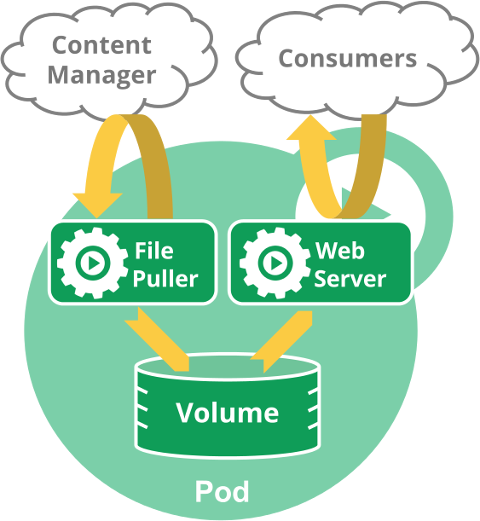
\includegraphics[width=300px]{../images/kubernetes/pod.png}
    \caption{Diagrama del ejemplo de dos contenedores en un mismo pod \protect\cite{k8spods}}
    \label{fig:k8s-pod}
\end{figure}

\subsubsection{Networking dentro de un Pod}
\label{subsubsec:networking-inside}

Dentro de un pod todos los contenedores están dentro del mismo namespace de red. Esto quiere decir que comparten asociaciones de puertos y se podrían pisar entre ellos si no elegimos bien y que se pueden comunicar mutuamente usando \emph{localhost}.

Kubernetes implementa este espacio de red compartido abriendo primero un contenedor que no hace nada y adjuntando los contenedores definidos en el pod a su red. Si entramos directamente en una de las máquinas y listamos los contenedores en ejecución veremos algunos con un nombre muy largo y acabados en el sufijo \emph{\_POD} que son los que refiero.

\subsubsection{Networking entre Pods}
\label{subsubsec:networking-between}

A cada pod se le asigna una IP privada única dentro del cluster. Cuando actualizamos o cerramos el pod se reasignará la dirección a otro, no es estática ni reservable con antelación. Mediante esta IP podemos contactar desde cualquier pod del cluster a cualquier otro, en la misma o en distintas máquinas. Más adelante veremos como ``reservar'' una IP para un servicio concreto (\ref{subsec:services}) y como usar nombres de host personalizados en lugar de IPs para facilitar la programación y configuración (\ref{subsec:addons-dns}).

\subsection{Etiquetas y selectores}
\label{subsec:labels-selectors}

Los pods se pueden etiquetar con parejas de \emph{clave, valor} que deseemos. Esta característica heredada de Borg nos permite mucha flexibilidad al seleccionar pods para otros componentes que veremos a continuación. Se pueden usar para filtrar listados, filtrar observadores de la API que se activan con los cambios o configurar componentes.

En la figura \ref{fig:k8s-labels-selectors} vemos por ejemplo dos selectores en blanco y como eligen los pods de color filtrando por sus etiquetas.

\begin{figure}[H]
    \centering
    \includegraphics[width=\textwidth]{../images/kubernetes/labels.png}
    \caption{Selección de pods}
    \label{fig:k8s-labels-selectors}
\end{figure}

Aunque pueda subestimarse fácilmente por parecer una idea simple es sin embargo un engranaje necesario para muchos de los comportamientos que vienen a continuación. La flexibilidad de poder seleccionar con un grano más fino o más grueso y agrupando ad-hoc es algo difícil de igualar en otras plataformas.

Las etiquetas se pueden usar en otros componentes que veremos (se pueden etiquetar servicios, replication sets, etc.) de la misma manera que con los pods. Especialmente interesante es el caso de los nodos que podemos etiquetar (y se hace por defecto) por tipo de disco o zona de disponibilidad con el objetivo de filtrar las máquinas en las que un pod puede ejecutarse satisfactoriamente.

\subsection{Replica Set}
\label{subsec:rs}

Un conjunto de réplicas genera una abstracción estable sobre la idea de pods efímeros. Un pod puede abrirse o cerrarse, pero un un RS tiene un solo nombre y debe eliminarse explícitamente si no lo necesitamos. En el conjunto se puede usar un selector de etiquetas para elegir que pods controla y un número de unidades objetivo. El sistema se encargará de mantener ese número exacto de pods abriendo o cerrando los que sean necesarios.

Si además damos un paso más ese objetivo puede variar dinámicamente a través de la API. Podemos usarlo para cambiar el número de instancias de nuestra aplicación de acorde a métricas que indiquen la carga que tiene, por ejemplo. Esto da lugar a un componente del que no hablaré que se llama Horizontal Pod Autoscaler.

Los RS son versiones avanzadas de un componente que se usaba con bastante frecuencia antes denominado \emph{Replication Controller}. El funcionamiento y características básicas son similares, aunque los RS pueden usar selectores basados en conjuntos \cite{k8slabelsset} que permiten usos más avanzados. Además las nuevas incorporaciones como los deployments usan directamente conjuntos en lugar de controladores.

\subsection{Deployment}
\label{subsec:deployment}

El último nivel de abstracción sobre los pods que se usa a nivel de administración para ejecutar las aplicaciones. Define una plantilla para los pods que se crearán asociada a un nombre estable elegido por el usuario.

El deployment se encarga de mantener el número de pods que le pidamos modificando internamente el objetivo del replica set que tiene por debajo y que gestiona automáticamente.

Este componente se encarga también de gestionar las actualizaciones asíncronamente de la forma menos disruptiva posible de acorde a dos posibilidades:
\begin{itemize}
  \item \textbf{Recrear}. Cuando actualizamos la plantilla del pod en el deployment éste comenzará un proceso para cerrar las instancias que tengamos y luego abrir las nuevas.
  \item \textbf{Actualización continua}. Al cambiar irá progresivamente reemplazando las instancias antiguas con las nuevas. Se puede controlar la velocidad de cambio y cuantos pods estamos dispuestos a encender/apagar al mismo tiempo durante el proceso.
\end{itemize}

Ambos tipos de actualizaciones son posibles gracias a los Replica Sets que gestiona el deployment internamente. El caso especialmente interesante es la actualización continua. Al guardar el cambio se genera un segundo RS. Posteriormente poco a poco se va reduciendo el objetivo del conjunto original para ir aumentándolo al mismo ritmo en el nuevo conjunto. Cuando todo esté correcto y migrado se puede eliminar el RS antiguo y el sistema está preparado para la siguiente actualización de la aplicación. Estos dos pasos se reflejan en las figuras \ref{fig:k8s-rolling-step1} y \ref{fig:k8s-rolling-step2}.

Esta manera de aplicar cambios progresivos sobre un deployment nos permite pausar o revertir el cambio en cualquier momento si detectamos fallos significativos de cara al usuario en la nueva versión. Cuando se arregle podemos continuar con la actualización o lanzar otra nueva sin problemas.

\begin{figure}[H]
    \centering
    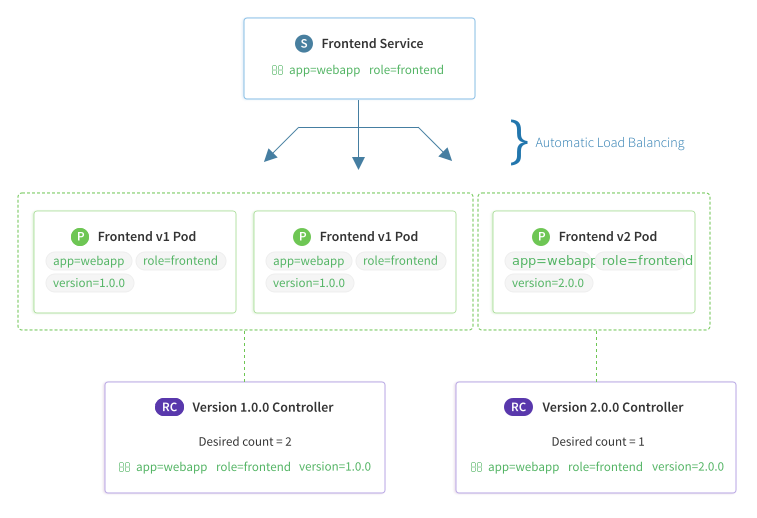
\includegraphics[width=\textwidth]{../images/kubernetes/rolling-deploy.png}
    \caption{1º paso: abrir un RS con la nueva versión\cite{coreosrc}}
    \label{fig:k8s-rolling-step1}
\end{figure}

\begin{figure}[H]
    \centering
    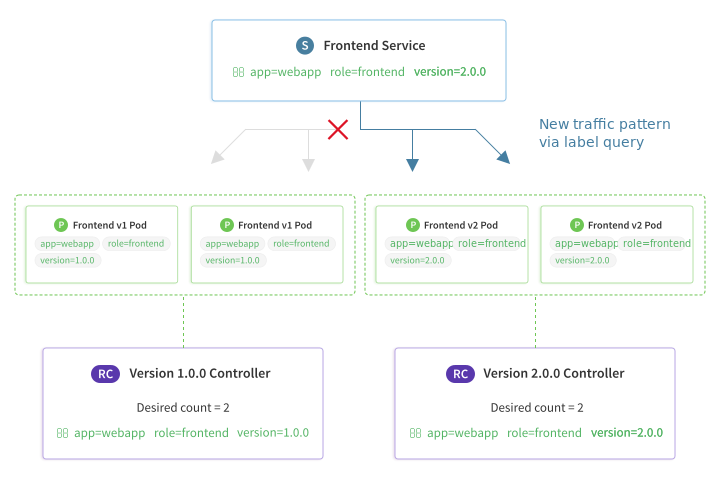
\includegraphics[width=\textwidth]{../images/kubernetes/traffic-shift.png}
    \caption{2º paso: migrar el tráfico lentamente al nuevo RS hasta terminar\cite{coreosrc}}
    \label{fig:k8s-rolling-step2}
\end{figure}

\subsection{Servicios}
\label{subsec:services}

Los servicios balancean las conexiones de red entre los pods que seleccionemos mediante etiquetas. Cada servicio lleva un nombre elegido por el usuario y una IP interna estable que no cambia durante su vida; ambas cosas permiten conectarse con él. Solo se exponen los puertos que pidamos explícitamente.

Además del balanceo interno podemos pedir que Kubernetes nos configure complementos externos automáticamente (el balanceador de carga de Google Cloud o AWS por ejemplo) para nos podamos conectar desde fuera. La alternativa para habilitar conexiones externas es pedir que el servicio escuche en un puerto concreto de todas las máquinas y configurar los balanceadores manualmente. Ésta última opción es necesaria en instalaciones directas sobre máquinas propias o Minikube (\ref{sec:minikube}).

Cuando nos conectamos a un servicio da igual a qué máquina lleguemos, \emph{kube-proxy} se encarga de redirigirnos a uno de los pods que implementen dicho servicio sin problemas.

\subsection{Namespaces}
\label{subsec:namespaces}

Kubernetes ha desarrollado algunas características para usos avanzados del sistema como los namespaces. Nos permiten agrupar y separar los pods, servicios, deployments y otros componentes que usemos. Un servicio o deployment puede por ejemplo tener el mismo nombre que otro siempre que estén en namespaces distintos. Al crear un nuevo componente se puede elegir el namespace que no cambiará durante la vida del objeto.

Aparte de permitir la gestión individual por usuario/equipo o lo que se necesite los namespaces habilitan el establecimiento de cuotas sobre los recursos. Podemos por ejemplo dedicar un 35\% de la memoria del cluster al equipo de análisis de datos y un 65\% al equipo de producción que mantiene la aplicación visible para el usuario final.

\subsection{Cuotas}
\label{subsec:quotas}

Existen cuotas para limitar los recursos que se pueden reservar y usar desde un namespaces. Los recursos comprenden un abanico de posibilidades desde métricas del propio nodo como memoria y CPU a métricas del sistema como número de pods\cite{k8squota}.

Se pueden usar estas cuotas para limitar el impacto que un cliente tuviera sobre los demás en caso de subir un código erróneo o demasiado pesado para el entorno.

\section{Addons}
\label{sec:addons}

Kubernetes distribuye con las instalaciones oficiales una serie de plugins o addons que pueden añadirse según se quiera al cluster. Se ejecutan como pods normales y corrientes sobre un namespace llamado \emph{kube-system} para que no molesten al usuario en un uso normal. Hay plugins para configurar el logging (FluentD, Graphite, etc.), registro de contenedores y monitorización por ejemplo. Voy a hablar especialmente el único addon que he usado: el DNS.

\subsection{Addon: DNS}
\label{subsec:addons-dns}

Todos los servicios se crean con un nombre elegido por el usuario. Este addon registra esos nombres asociados a las IPs en un servidor DNS configurable llamado SkyDNS\cite{skydns}. Todos los pods llevan configurado ese servidor como servidor DNS principal. Si pedimos un dominio de la forma ``[nombre]'' si estamos en el mismo namespace o ``[nombre].[namespace].svc.cluster.local'' si queremos ser explícitos podemos obtener la IP del servicio para comunicarnos con él. Si pedimos cualquier otro dominio la petición se redirecciona al servidor DNS primario que tuvieran las máquinas del cluster configurado.

Este addon facilita la comunicación entre distintos microservicios del sistema usando un nombre estable y elegido por el usuario sin tener que preocuparse por la topología y las direcciones IP elegidas individualmente para cada servicio y pod. Desacopla la programación de la administración del sistema facilitando el trabajo de ambos equipos.

\subsection{Addon: Dashboard}
\label{subsec:addon-dashboard}

Otro complemento bastante útil es una aplicación web denominada Dashboard que consulta la API para ofrecernos una interfaz intuitiva y online para la administración del cluster. Proporciona mecanismos para crear nuevos componentes y nos lista los deployments, pods, servicios, etc. que tengamos. Además recopila métricas de rendimiento (CPU y memoria) para trazar pequeños gráficos de la evolución y estado del sistema a corto plazo.

\section{Minikube}
\label{sec:minikube}

Los desarrolladores de Kubernetes han preparado una aplicación independiente para ayudar a configurar un entorno local que reproduzca el entorno de producción lo más fielmente posible. Minikube es capaz de configurar una máquina virtual con VirtualBox o VMWare y el demonio de Docker ya instalado usando Docker Machine\cite{dockermachine}. Dentro de esa máquina instala los 5 demonios de Kubernetes.

Podemos acceder al cluster a través de la línea de comandos con las configuraciones que se añaden automáticamente a \emph{kubectl} o llamando a la API con la IP de la máquina que nos devuelve Minikube al configurarla.

El ``cluster'' local que hemos montado funciona casi igual a uno real a excepción de algunas diferencias lógicas\cite{minikube}:
\begin{itemize}
  \item Hay un solo nodo registrado. No se pueden probar cosas que impliquen la programación de pods en varios nodos, por ejemplo para alta disponibilidad.
  \item No hay ningún balanceador de carga en la nube que configurar. Si queremos acceder a un servicio debemos exponerlo en un puerto del nodo y usar la IP de la máquina virtual.
  \item Al usar Docker Machine es imposible probar servicios de contenedores alternativos como Rocket.
\end{itemize}

\section{Alternativas}
\label{sec:k8s-alternativas}

\subsection{OpenShift}
\label{subsec:k8s-alternativas-openshift}

OpenShift está basado en Kubernetes, de hecho muchos de los ingenieros que colaboran en un proyecto lo hacen frecuentemente en el otro. Además de los componentes básicos que ya existen en el sistema OpenShift añade algunos más interesantes desde el punto de vista empresarial, como son autenticación por LDAP, enrutamiento avanzado de red o sistemas de control por permisos más avanzados. La mayor parte de estas mejoras están en camino o se incorporarán en algún momento en el proyecto padre Kubernetes, la colaboración es continua y sostenida en el tiempo.

He decidido usar Kubernetes porque no necesitaba ninguna de esas caaracterísticas avanzadas y estoy más familiarizado con sus comandos.

\subsection{Nomad}
\label{subsec:k8s-alternativas-nomad}

Nomad\cite{nomad} es un sistema para controlar las aplicaciones de un cluster. Llega mucho más allá de los contenedores y está preparado para ejecutar aplicaciones planas como J2EE sobre un servidor web como Tomcat o un binario cualquiera. Está desarrollado por una empresa llamada Hashicorp\cite{hashicorp} que tiene bastante buena fama entre los desarrolladores por productos estables y útiles como Vagrant (control de máquinas virtuales por scripts de Ruby), Packer (construir imágenes de máquinas virtuales), Consul (similar a etcd, base de datos distribuida para clave, valor) y Terraform (gestión de clústeres en AWS).

No he usado Nomad porque la gestión de volúmenes de Docker no la tienen bien solucionada todavía\cite{nomdadvolumesbug} y tampoco tienen ninguna abstracción de red como los servicios de Kubernetes para balancear la carga automáticamente entre trabajos.

\subsection{Swarm}
\label{subsec:k8s-alternativas-swarm}

Swarm\cite{swarm} es un servicio integrado en Docker que proporciona control de cluster con las mismas llamadas y directivas que se usan para controlar una sola máquina. Mediante los plugins de volúmenes y un DNS integrado en el propio servidor de contenedores puede ofrecer características parecidas a los volúmenes y red de Kubernetes.

No lo he utilizado por varias razones:
\begin{itemize}
  \item La instalación en un entorno de desarrollo es totalmente manual.
  \item La API cambia constantemente a cada nueva versión de Docker.
  \item Carece de un modo sencillo de crear nuevas aplicaciones y actualizarlas como los deployments de Kubernetes.
\end{itemize}
